\documentclass[conference]{IEEEtran}

\usepackage{amsmath, amssymb}
\usepackage{graphicx}
\usepackage{cite}
\usepackage{booktabs}
\usepackage{hyperref}
\usepackage{enumitem}
\usepackage{array}
\usepackage{makecell}

\begin{document}
	
	\title{Reproducible 6-DOF Wrist-Roll Retrofit for OpenMANIPULATOR-X}
	
	\author{
		\IEEEauthorblockA{
			Author names withheld for double-blind review\\
			Affiliation withheld for double-blind review\\
			Email withheld for double-blind review}
	}
	
	\maketitle
	
	\begin{abstract}
		Low-cost educational manipulators lack the full orientation control
		required for complex manipulation tasks due to their limited degrees
		of freedom. This paper presents a reproducible retrofit that upgrades
		the OpenMANIPULATOR-X from a 5-DOF to a 6-DOF system by integrating an
		additional wrist-roll joint, together with a unified ROS~2/MoveIt~2
		software stack and an open hardware kit. A pose-based benchmarking
		framework compares the 5-DOF and 6-DOF configurations under identical
		conditions across kinematic feasibility, constrained-corridor
		planning, and physical hardware execution.
		
		Results show the 6-DOF arm achieves complete reachability across the
		tested orientation set (7/7) versus 1/7 for the 5-DOF baseline. In a
		constrained corridor at the narrowest tested width, the 6-DOF
		configuration achieves a 24.3\% planning success rate versus 0.0\%
		for the 5-DOF system ($\chi^2(1){=}17.14$, $p{=}3.5{\times}10^{-5}$,
		Cohen's $h{=}1.031$), with success rising above 80\% at moderate
		corridor widths. Hardware validation on 120 poses, performed on a
		single retrofitted hardware prototype, shows the retrofit preserves
		orientation fidelity on physical hardware (97.5\% success within
		$5^\circ$, mean error $1.89^\circ$) despite a larger, honestly
		quantified Cartesian position gap (40\% strict success within
		5\,mm). The complete hardware and software design is released as an
		open, low-cost (${\approx}\$58$ incremental) upgrade path intended
		to support replication by other laboratories; reproducibility
		claims in this paper refer to the design and software artifacts,
		while hardware results reflect validation on the single physical
		prototype described above.
	\end{abstract}
	
	\begin{IEEEkeywords}
		Degrees of freedom, robot kinematics, OpenMANIPULATOR-X, wrist-roll
		retrofit, ROS~2, MoveIt~2, motion planning, benchmarking.
	\end{IEEEkeywords}
	
	% ============================================================
	\section{Introduction}
	\label{sec:introduction}
	% ============================================================
	
	Low-cost educational manipulators such as the OpenMANIPULATOR-X
	\cite{robotis2023openmanipulator} are widely used with ROS~2
	\cite{al2024ros} and MoveIt~2 \cite{chitta2016moveit} for instruction
	and prototyping, but their standard 5-DOF configuration lacks an
	independent wrist-roll joint, restricting the orientations achievable
	at a fixed end-effector position. This constrains tasks requiring
	precise alignment or orientation-controlled manipulation, where
	compensatory joint motions increase execution time and reduce
	planning success. Six independent DOF are theoretically required
	for arbitrary end-effector pose (position and orientation)
	\cite{craig2005introduction, whitney1969resolved}; at a fixed
	position, achieving arbitrary orientation specifically requires an
	independently actuated wrist-roll axis. This requirement's practical
	impact on low-cost platforms is rarely characterized under
	controlled, reproducible conditions.
	
	This paper presents a fully reproducible 6-DOF wrist-roll retrofit
	for the OpenMANIPULATOR-X: mechanical integration, an updated
	URDF/Xacro model, \texttt{ros2\_control} and MoveIt~2 configuration,
	and a pose-based benchmarking framework comparing 5-DOF and 6-DOF
	configurations under identical conditions.
	
	\textbf{Contributions:}
	\begin{itemize}[leftmargin=*,itemsep=1pt,topsep=2pt]
		\item A low-cost (${\approx}\$58$ incremental) 6-DOF wrist-roll
		retrofit with open, reproducible hardware and software artifacts,
		validated in simulation and on a single physical prototype.
		\item A pose-based benchmarking framework that isolates the
		effect of the added DOF across IK feasibility, constrained
		planning, and hardware execution.
		\item Statistically grounded evidence (chi-square, effect sizes,
		confidence intervals) of the retrofit's benefit, together with
		an honest, quantified sim-to-real comparison.
	\end{itemize}
	
	Section~II reviews related work; Section~III describes the retrofit;
	Section~IV details the methodology; Section~V reports results;
	Section~VI discusses implications; Section~VII concludes.
	
	% ============================================================
	\section{Related Work}
	\label{sec:related_work}
	% ============================================================
	
	Manipulators spanning a range of cost and capability — from
	low-cost platforms such as OpenMANIPULATOR-X
	\cite{robotis2023openmanipulator} and WidowX \cite{zhao2021widowx} to
	research-grade arms such as the Franka Panda \cite{franka2023panda} —
	are widely used in robotics education and research
	\cite{muepu2025toward}; among the low-cost tier, 5-DOF platforms
	face inherent orientation-coverage limits, discussed further below.
	Six DOF are required for arbitrary end-effector pose
	\cite{craig2005introduction}, and the absence of an independent
	wrist-roll joint is known to prevent full orientation specification
	\cite{craig2005introduction, whitney1969resolved}; this limitation is,
	however, typically discussed qualitatively rather than characterized
	experimentally on widely used low-cost hardware. Modern manipulation
	stacks build on ROS~2 \cite{macenski2022ros2control},
	\texttt{ros2\_control}, and MoveIt~2 \cite{chitta2016moveit}, with
	OMPL \cite{sucan2012ompl} providing sampling-based planners,
	Planner Arena \cite{plannerarena} supporting systematic benchmarking
	of planning algorithms, and standardized protocols such as those of
	Falco~\textit{et al.} \cite{norton2020developing} supporting
	systematic benchmarking of manipulator and end-effector performance
	more broadly. Constraint-aware planning in narrow or cluttered
	environments has
	been studied by Berenson~\textit{et al.} \cite{berenson2011task},
	highlighting the role of manipulator dexterity under geometric
	restriction. Reproducibility-focused efforts such as Meta-World
	\cite{benchmarkrobotlearning} emphasize sharing complete experimental
	artifacts; however, prior low-cost-manipulator retrofits typically
	report hardware augmentation without a fully integrated,
	statistically validated evaluation pipeline. This work addresses that
	gap by combining a documented mechanical/software retrofit with a
	controlled, pose-based statistical comparison.
	
	% ============================================================
	\section{System Design}
	\label{sec:system}
	% ============================================================
	
	\subsection{Mechanical Retrofit}
	
	A single revolute joint is added between the wrist-pitch link
	(\textit{link5}) and the gripper assembly, actuated by a Dynamixel
	XL430-W250-T servo (ID~15; the existing gripper servo is reassigned
	to ID~16 to avoid conflicts). This achieves independent end-effector
	roll without modifying the five existing joints, at an incremental
	hardware cost of ${\approx}\$58$ (Table~\ref{tab:bom}) and
	${\approx}1$~hour of fully reversible assembly; both structural adapters
	are 3D-printable, and STL/STEP files are provided in the project
	repository (link withheld for double-blind review; released upon
	publication).
	
	\begin{table}[t]
		\centering
		\caption{Incremental Bill of Materials (6-DOF Retrofit)}
		\label{tab:bom}
		\small
		\begin{tabular}{lll}
			\toprule
			\textbf{Component} & \textbf{Qty} & \textbf{Notes} \\
			\midrule
			Dynamixel XL430-W250-T & 1 & Wrist-roll actuator, ID~15 \\
			Wrist link + gripper bracket & 2 & 3D-printed adapters \\
			Fasteners + RS-485 cable & --- & Standard hardware \\
			\midrule
			\multicolumn{3}{l}{\textbf{Total incremental cost:} ${\approx}$5,599 INR (${\approx}\$58$)} \\
			\bottomrule
		\end{tabular}
	\end{table}
	
	\subsection{Software Integration}
	
	The URDF/Xacro kinematic chain was extended with a revolute joint
	(axis $[1,0,0]$, limits $\pm\pi$~rad) between \textit{link5} and a
	new \texttt{wrist\_roll\_link}, with downstream gripper and TCP
	frames re-parented accordingly. The \texttt{ros2\_control} hardware
	interface, transmission matrices, and controller configuration were
	expanded from five to six joints, and the MoveIt~2 SRDF, joint
	limits, and controller lists were updated to include
	\texttt{joint5\_roll} in the arm planning group. A GUI panel and CSV
	logging were extended to expose the new joint. All modifications and
	per-commit diffs are available in the project repository for full
	reproducibility.
	
	% ============================================================
	\section{Methodology}
	\label{sec:methodology}
	% ============================================================
	
	\subsection{Pose-Based Evaluation and Workspace Estimation}
	
	Initial joint-space sampling was found to unfairly favor the 6-DOF
	arm's larger configuration space; evaluation was therefore switched
	to a pose-based framework in which both arms are compared on their
	ability to reach identical target end-effector poses. Each
	configuration's reachable workspace was estimated via
	forward-kinematics sampling (convex-hull and alpha-shape boundaries,
	Fig.~\ref{fig:workspace}), and the intersection of the two workspaces
	was used to constrain all subsequent pose generation, so that every
	evaluated pose is reachable by both arms independent of positional
	workspace differences. The alpha-shape parameter and forward-kinematics
	sampling density used to estimate each workspace are documented in the
	project repository to enable exact reproduction.
	
	\begin{figure}[t]
		\centering
		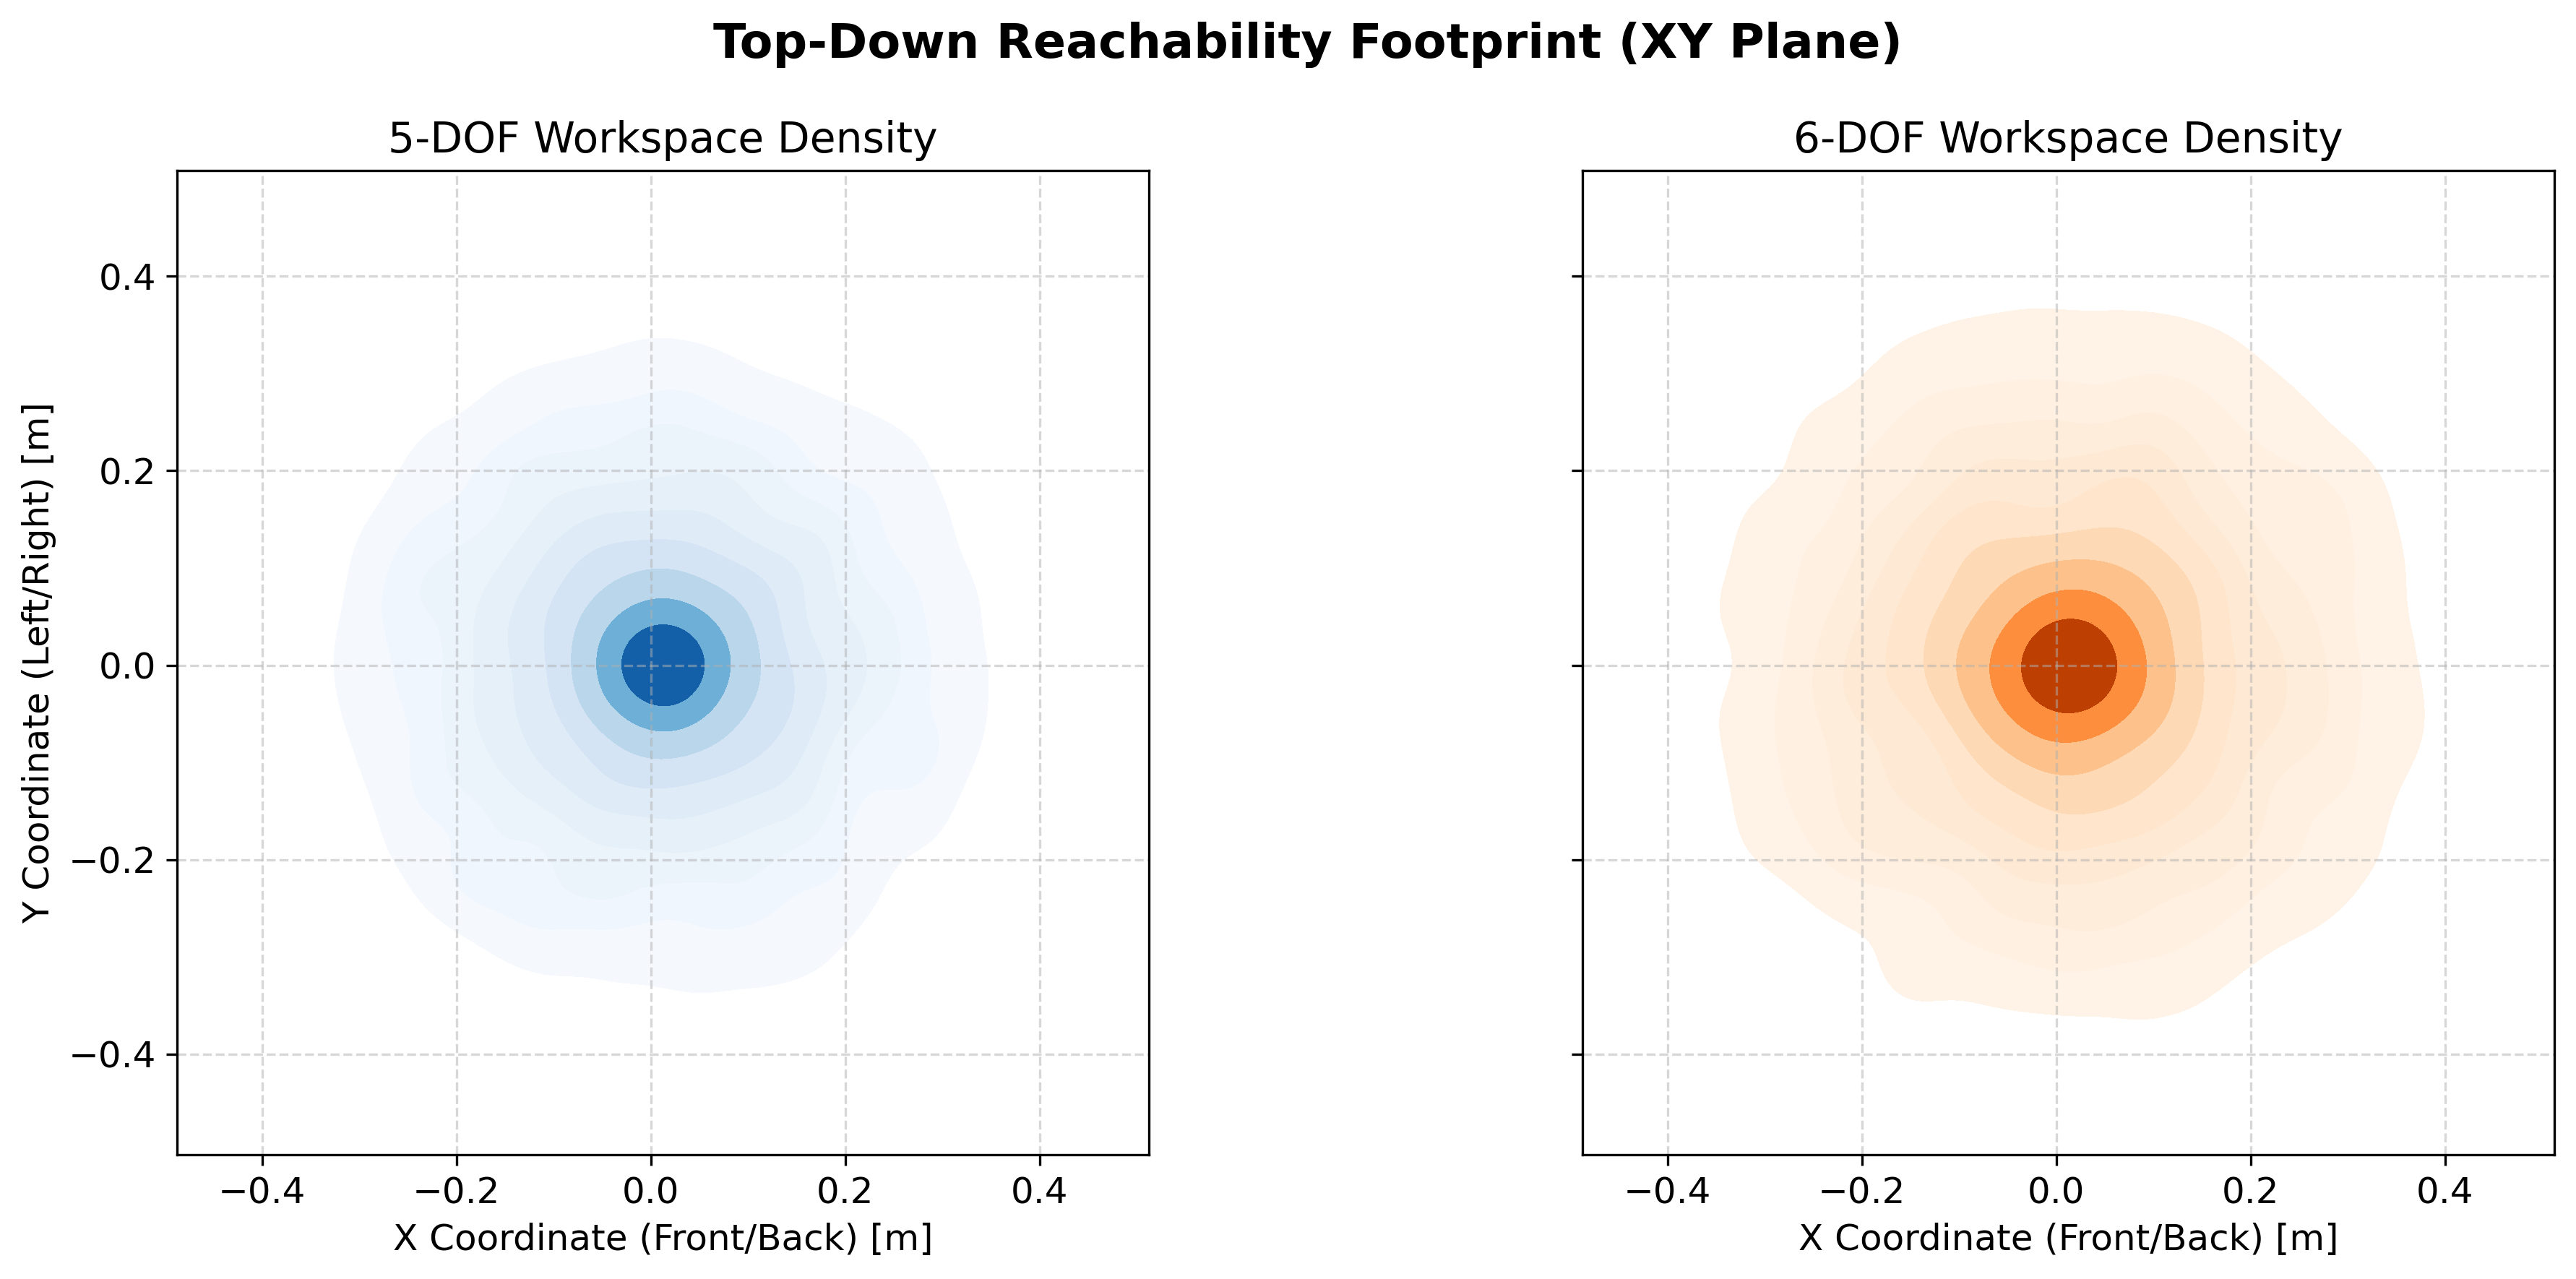
\includegraphics[width=0.85\linewidth]{figures/workspace_comparasion_TopDown_Heatmaps.png}
		\caption{Shared reachable workspace (top-down density) used to
			constrain all evaluation poses for both configurations.}
		\label{fig:workspace}
	\end{figure}
	
	\subsection{Orientation Reachability Protocol}
	
	At a fixed, collision-free position $(0.20, 0.00, 0.15)$~m within the
	shared workspace, seven pure-roll orientations
	($0^\circ$--$90^\circ$, $15^\circ$ steps) were evaluated via the
	MoveIt~2 IK service, isolating IK feasibility from motion-planning
	effects. This discrete grid characterizes coverage trends across a
	single rotational axis rather than certifying continuous
	full-orientation feasibility; denser or higher-dimensional sampling
	is left to future work.
	
	\subsection{Constrained-Corridor Planning Benchmark}
	
	A narrow corridor scene was built in the MoveIt~2 planning scene,
	with width swept over five values (0.24--0.40~m) to characterize
	planning success as a function of spatial constraint
	(Fig.~\ref{fig:corridor}). At each width, goal poses were restricted
	to the IK-feasible set from IV-B, and planning was performed with
	OMPL RRTConnect (10~s limit, 10 trials per goal) to account for
	planner stochasticity, a sample size consistent with common practice
	in OMPL/MoveIt~2 benchmarking studies for characterizing binary
	success rates under repeated stochastic planning attempts. At the
	narrowest tested width, both configurations were evaluated over 7
	feasible goals $\times$ 10 trials/goal (70 trials), giving a directly
	comparable sample size across the two configurations.
	
	\subsection{Cross-Configuration Kinematic Compatibility}
	
	With collision checking disabled, two independent sets of
	${\sim}8{,}000$ end-effector poses were generated via
	forward-kinematics sampling of each arm's own joint space (Halton
	low-discrepancy sequence) and evaluated for IK solvability on
	\emph{both} arms. IK solvability was evaluated with the same
	MoveIt~2 IK service and solver tolerance settings used elsewhere in
	this study; exact position and orientation tolerance values are
	fixed in the solver configuration file released in the project
	repository, allowing exact reproduction without restating them
	here. This
	large sample is used to densely characterize the shape of each arm's
	reachable-orientation manifold, and is distinct from the smaller,
	trial-based samples in Section~V used for planning-success hypothesis
	testing. Because the 5-DOF arm's feasible roll at any fixed position
	is a single value, while poses in this test are drawn from a
	continuous $\pm\pi$~rad range, near-zero overlap between the two
	sampled manifolds is the expected outcome under a tight IK tolerance
	almost by construction — analogous to asking how many points drawn
	uniformly from a cube land exactly on one face — rather than an
	inherently surprising empirical result.
	
	\subsection{Statistical Framework}
	
	Pearson's $\chi^2$ test, Cramer's $V$, Cohen's $h$, and Wilson-score
	95\% confidence intervals were applied to binary planning-success
	outcomes; Welch's $t$-test/Cohen's $d$ were used for planning-time
	comparisons. Cohen's $h$ was computed via the arcsine-transform
	formula, $h = 2\arcsin(\sqrt{p_1}) - 2\arcsin(\sqrt{p_2})$, so that
	the reported value can be verified directly from the two reported
	proportions. Given a zero-count cell in the corridor-planning
	comparison (Table~\ref{tab:corridor_stats}), Yates' continuity-corrected
	$\chi^2$ was used; the uncorrected $\chi^2$ statistic for the same
	table is higher (${\approx}19.35$). All computations used Python
	(NumPy/SciPy).
	
	\subsection{Hardware Validation Protocol}
	
	A set of 120 validation poses (Halton sampling, then boundary/interior
	stratification via Farthest Point Sampling) was executed on both the
	simulated and physical retrofitted arm under identical
	\texttt{ros2\_control} trajectory interfaces, recording joint
	tracking error, Cartesian position error, orientation error, and
	repeatability for direct sim-to-real comparison. All hardware
	results in Section~V-E were collected on a single retrofitted
	physical unit; see the Limitations paragraph in Section~VI for the
	scope this implies.
	
	% ============================================================
	\section{Results}
	\label{sec:results}
	% ============================================================
	
	\subsection{Orientation Reachability}
	
	\begin{table}[t]
		\centering
		\caption{IK Feasibility by Roll Orientation}
		\label{tab:ik}
		\small
		\begin{tabular}{lcccccccc}
			\toprule
			\textbf{Config.} & $0^\circ$ & $15^\circ$ & $30^\circ$ & $45^\circ$ & $60^\circ$ & $75^\circ$ & $90^\circ$ & \textbf{Total} \\
			\midrule
			5-DOF & \checkmark & $\times$ & $\times$ & $\times$ & $\times$ & $\times$ & $\times$ & 1/7 \\
			6-DOF & \checkmark & \checkmark & \checkmark & \checkmark & \checkmark & \checkmark & \checkmark & 7/7 \\
			\bottomrule
		\end{tabular}
	\end{table}
	
	The 5-DOF arm achieves a feasible IK solution only at $0^\circ$ roll
	— a structural rather than algorithmic limitation, since no IK
	solution exists for non-zero roll at a fixed position without an
	independent wrist-roll joint. The 6-DOF arm achieves complete
	reachability across the tested orientation set, a $7\times$ increase
	in coverage ($14.3\%\rightarrow100\%$), consistent with the
	theoretical requirement of six independent DOF for arbitrary
	end-effector pose \cite{craig2005introduction, whitney1969resolved},
	of which the added roll axis specifically enables orientation
	coverage at a fixed position.
	
	\subsection{Cross-Configuration Kinematic Compatibility}
	
	\begin{table}[t]
		\centering
		\caption{Cross-Configuration Kinematic Compatibility}
		\label{tab:cross}
		\small
		\begin{tabular}{lccc}
			\toprule
			\textbf{Condition} & \textbf{Poses} & \textbf{Solved} & \textbf{Rate} \\
			\midrule
			5-DOF $\rightarrow$ 5-DOF (self)  & 7339 & 6908 & 94.13\% \\
			6-DOF $\rightarrow$ 5-DOF (cross) & 7239 &    0 &  0.00\% \\
			\midrule
			\multicolumn{3}{l}{Shared kinematic space} & 0.00\% \\
			\multicolumn{3}{l}{Dexterity expansion (6-DOF vs.\ 5-DOF)} & 100.00\% \\
			\bottomrule
		\end{tabular}
	\end{table}
	
	Because the 5-DOF arm's feasible roll at any fixed position is a
	single value, while the 6-DOF-sampled poses are drawn from a
	continuous $\pm\pi$~rad range, near-zero overlap between the two
	manifolds is the expected outcome of this sampling design under a
	tight IK tolerance (Section~IV-D) — not, on its own, a surprising
	empirical finding. Consistent with that expectation, the 5-DOF arm
	solves 94.13\% of its own densely-sampled poses (confirming solver
	reliability) but 0\% of the ${\sim}7{,}239$ poses drawn from the
	6-DOF arm's manifold: no sampled 6-DOF pose was jointly IK-solvable
	by the 5-DOF arm under our solver tolerance. This corroborates,
	rather than independently establishes, the orientation-reachability
	result of Section~V-A, and confirms the same effect holds under
	dense sampling of the full manifold rather than only at the seven
	discrete test orientations.
	
	We summarize this as a \emph{Shared Kinematic Space} of 0\% (the
	fraction of the 6-DOF-sampled set also solvable by the 5-DOF arm)
	and a \emph{Dexterity Expansion} of 100\% (Table~\ref{tab:cross}).
	Given the sampling argument above, these bounds are expected rather
	than a novel discovery; we report them as a compact, quantified
	summary of the manifold comparison, relative to the sampled pose set
	and stated solver tolerance, not as a universal property of the two
	kinematic chains.
	
	\subsection{Constrained-Corridor Planning}
	
	\begin{figure}[t]
		\centering
		% NOTE: The source image must show the 6-DOF success rate at the
		% narrowest width (0.24 m) as 24.3% to match the exact value
		% (17/70) reported in Table III and the body text below. If the
		% currently rendered figure shows a different value, it must be
		% regenerated from the corrected data before submission; this is
		% a plot-regeneration fix and cannot be patched from the LaTeX
		% source alone.
		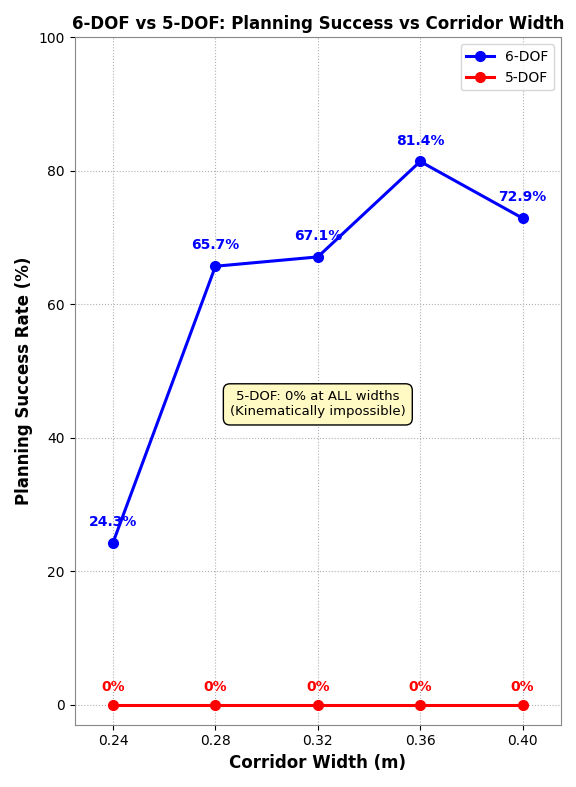
\includegraphics[width=0.85\linewidth]{figures/success_rate_constrained_various_corridor_widths.png}
		\caption{6-DOF vs.\ 5-DOF planning success across the full
			corridor-width sweep (0.24--0.40~m).}
		\label{fig:corridor}
	\end{figure}
	
	\begin{table}[t]
		\centering
		\caption{Corridor Planning Results (Width 0.24\,m) and Statistics}
		\label{tab:corridor_stats}
		\small
		\begin{tabular}{lccc}
			\toprule
			\textbf{Config.} & \textbf{Trials} & \textbf{Successes} & \textbf{Rate (95\% CI)} \\
			\midrule
			6-DOF & 70 & 17 & 24.3\% (15.8--35.5\%) \\
			5-DOF & 70 &  0 &  0.0\% (0.0--5.2\%) \\
			\bottomrule
		\end{tabular}
		\vspace{2pt}
		\small $\chi^2(1){=}17.14$ (Yates-corrected), $p{=}3.5{\times}10^{-5}$;
		Cramer's $V{=}0.350$; Cohen's $h{=}1.031$.
	\end{table}
	
	At the narrowest tested width (0.24~m), the $0^\circ$-roll goal — the
	only orientation kinematically reachable by the 5-DOF arm — yields
	0\% planning success for \emph{both} arms, indicating that the
	6-DOF advantage at this width is entirely attributable to planning
	success at non-zero-roll goals, which are exclusively reachable by
	the 6-DOF configuration. The 24.3\% headline figure therefore
	reflects a deliberately conservative (narrowest) test condition
	rather than the platform's best-case planning performance.
	
	As shown in Fig.~\ref{fig:corridor}, success rises with corridor
	width for both configurations, peaking at 81.4\% for the 6-DOF arm
	at 0.36~m before a slight decline at the widest tested setting
	(0.40~m, 72.9\%); a plausible mechanistic explanation for this
	non-monotonic trend is discussed in Section~V-D, though it was not
	directly measured in this study. The chi-square test rejects
	independence between configuration and planning success
	($p{=}3.5{\times}10^{-5}$), and Cohen's $h{=}1.031$ places the effect
	in the large category.
	
	\subsection{Joint Utilization}
	
	\begin{figure}[t]
		\centering
		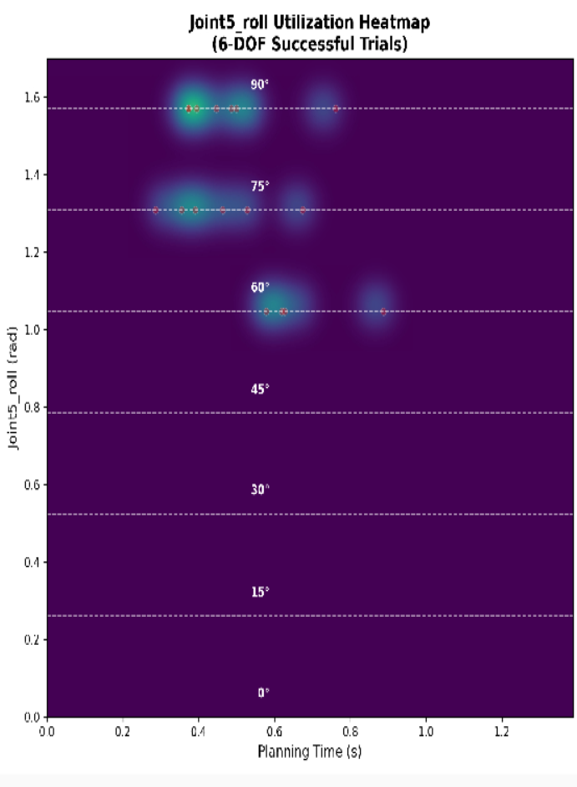
\includegraphics[width=0.85\linewidth]{figures/joint5_heatmap_6dof_success_trials.png}
		\caption{Distribution of \texttt{joint5\_roll} values across
			successful 6-DOF trajectories, confirming active use of the
			added joint.}
		\label{fig:heatmap}
	\end{figure}
	
	Analysis of successful 6-DOF trajectories (Fig.~\ref{fig:heatmap})
	shows \texttt{joint5\_roll} values spread broadly across the
	$\pm\pi$~rad range, with no successful trajectory holding the joint
	near zero throughout execution — confirming the planner genuinely
	exploits the added DOF rather than leaving it kinematically passive.
	Successful trials are concentrated at the higher-roll orientations
	($60^\circ$--$90^\circ$); at low roll ($0^\circ$--$45^\circ$),
	planning success is negligible regardless of corridor width. We
	hypothesize that this pattern reflects corridor geometry: at high
	roll, \texttt{joint5\_roll} likely turns the gripper approximately
	parallel to the corridor walls, reducing its effective distal
	cross-section and opening collision-free approach trajectories that
	would otherwise remain geometrically blocked when the gripper is
	held perpendicular to the walls. Widening the corridor would then
	further relax this constraint, which may explain why planning
	success continues to rise with corridor width even though the
	underlying benefit originates from orientation, not clearance,
	freedom. This explanation is consistent with the observed
	roll-success correlation, but we did not directly measure collision
	geometry, approach angle, or roll-conditioned clearance statistics
	in this study; confirming it quantitatively is left to future work.
	
	\subsection{Hardware Validation}
	
	\begin{table}[t]
		\centering
		\caption{Hardware Validation: Simulation vs.\ Real Robot (120 Poses)}
		\label{tab:hw}
		\small
		\begin{tabular}{lccc}
			\toprule
			\textbf{Metric} & \textbf{Sim} & \textbf{Real} & \textbf{Gap} \\
			\midrule
			Strict position success ($<$5\,mm) & 100.0\% & 40.0\% & $-$60.0\,pp \\
			Orientation success ($<$5$^\circ$) & 100.0\% & 97.5\% & $-$2.5\,pp \\
			Mean Cartesian error & 0.050\,mm & 7.849\,mm & $\times$156 \\
			Boundary success rate & 100.0\% & 19.44\% & $-$80.6\,pp \\
			Interior success rate & 100.0\% & 48.81\% & $-$51.2\,pp \\
			Repeatability ($\sigma$) & $\pm$0.0055\,mm & $\pm$1.032\,mm & $\times$188 \\
			Mean angular error & $0.014^\circ$ & $1.888^\circ$ & $\times$135 \\
			\bottomrule
		\end{tabular}
	\end{table}
	
	Simulation achieves near-numerical-precision position accuracy, while
	the physical arm's mean Cartesian error is 7.85\,mm (40.0\% strict
	success within 5\,mm), attributable to Dynamixel gear backlash,
	structural compliance, and gravity loading — factors absent from the
	idealized model. Boundary poses, which impose higher joint torque,
	show a lower success rate (19.44\%) than interior poses (48.81\%),
	consistent with this interpretation. Despite the position gap,
	orientation fidelity is well preserved on hardware: 97.5\% of
	executions satisfy the $5^\circ$ constraint, with a mean angular
	error of only $1.89^\circ$. Repeatability ($\pm$1.03\,mm) falls
	within the range reported for comparable Dynamixel-based platforms.
	All figures in this subsection reflect a single physical retrofit
	unit (Section~IV-F); cross-unit variance is not characterized here.
	
	% ============================================================
	\section{Discussion}
	\label{sec:discussion}
	% ============================================================
	
	The IK-feasibility, cross-configuration, and corridor-planning
	results provide consistent evidence for the same underlying
	structural effect: removing wrist roll eliminates feasibility for
	non-zero-roll goals. The corridor result is the one that translates
	this into a task-level planning benefit rather than a purely
	kinematic one, and — as Fig.~\ref{fig:corridor} shows — this benefit
	strengthens substantially as spatial constraint is relaxed, a trend
	consistent with the hypothesized high-roll-orientation mechanism
	discussed in Section~V-D, though that mechanism itself was not
	directly measured.
	
	The hardware results distinguish two failure modes with different
	practical weight. Position accuracy on the physical arm is
	meaningfully worse than in simulation, largely due to actuator-class
	factors (Dynamixel backlash, compliance) rather than the retrofit
	itself. Orientation accuracy — the specific capability this retrofit
	adds — degrades far less, since \texttt{joint5\_roll} is a compact,
	distal joint that carries less load than the proximal shoulder and
	elbow joints. For applications where the primary benefit sought is
	orientation freedom, the physical arm delivers it at an operationally
	useful level.
	
	\textbf{Practical implications.} Within the evaluated
	orientation-reachability and corridor-planning benchmarks, the
	additional DOF determines whether the tested goals are reachable at
	all, rather than merely improving performance on goals reachable by
	both configurations; extending this to concrete manipulation tasks
	(e.g., insertion, cap alignment) is left to future work. The retrofit
	is low-cost (${\approx}\$58$, ${\approx}1$~hour) and fully documented
	in open artifacts, supporting replication.
	
	\textbf{Limitations.} Hardware validation was performed on a single
	physical unit; inter-unit variance from manufacturing tolerance and
	per-unit calibration is not characterized, so the reproducibility
	claim in this paper applies to the design and software, not yet to
	cross-unit hardware performance. Statistical treatment of the
	hardware results (Table~\ref{tab:hw}) is limited to point estimates
	and standard deviations rather than the confidence-interval framework
	used for the planning results; extending it is straightforward future
	work. The Shared Kinematic Space and Dexterity Expansion figures in
	Section~V-B are reported relative to the sampled pose set and stated
	IK tolerance rather than as universal properties of the two
	kinematic chains. The corridor-planning mechanism proposed in
	Section~V-D is a hypothesis consistent with the observed data, not a
	directly measured collision-geometry result. Finally, this study
	benchmarks the retrofit only against its own 5-DOF baseline; a
	direct comparison with existing commercial 6-DOF educational
	manipulators is left to future work.
	
	% ============================================================
	\section{Conclusion}
	\label{sec:conclusion}
	% ============================================================
	
	This work presented a low-cost, reproducible 6-DOF wrist-roll
	retrofit for the OpenMANIPULATOR-X and evaluated it through kinematic
	analysis, statistically grounded planning benchmarks, and hardware
	validation. The retrofit expands orientation coverage from 14.3\% to
	100\% and improves constrained-corridor planning success from 0.0\%
	to 24.3--81.4\% depending on spatial constraint, while preserving
	orientation fidelity on physical hardware. Future work will evaluate
	roll-critical manipulation tasks (insertion, alignment), extend the
	statistical framework to hardware validation, and assess a second
	physical build for cross-unit reproducibility.
	
	% ============================================================
	% ACKNOWLEDGMENT / AI USAGE DISCLOSURE
	% ------------------------------------------------------------
	% Grammar/language-editing-only use. Per IEEE PSPB policy, this
	% falls under "editing and grammar enhancement," which is
	% "generally outside the intent" of the mandatory AI-disclosure
	% rule — disclosure is recommended rather than required, so no
	% specific AI system is named here. If AI was used for anything
	% beyond grammar (e.g. drafting analysis text, verifying stats,
	% generating code), this statement must be expanded and the tool
	% named per IEEE policy.
	% ============================================================
	\section*{Acknowledgment}
	Generative AI tools were used to assist with grammar and language
	editing of the manuscript text. All experimental design, data
	collection, statistical analysis, and conclusions are the authors'
	own.
	
	\bibliographystyle{IEEEtran}
	\bibliography{references2}
	
\end{document}